\documentclass{article}

\newcommand\tab[1][1cm]{\hspace*{#1}}
\usepackage{graphicx}
\usepackage{epsfig}
\usepackage{wrapfig}
\usepackage{algorithm}
\usepackage{algorithmic}
\usepackage{amsmath}
\usepackage{makeidx}
\graphicspath{ {images/} }
\usepackage{scrextend}
\makeatletter
\let\@addmarginORIG\@addmargin
\renewcommand*\@addmargin{%
	\vspace{-\bigskipamount}
	\@addmarginORIG}
\makeatother
\usepackage{geometry}
\geometry{
	a4paper,
	total={140mm,237mm},
	left=30mm,
	top=30mm,
	bottom=30mm,
	right=30mm
}

\newenvironment{tightcenter}{%
	\setlength\topsep{0pt}
	\setlength\parskip{0pt}
	\begin{center}
	}{%
\end{center}
}

\author{Andrea Zampieri}
\title{Network Inference from Node Embedding:\newline Deep Autoencoding}


\begin{document}
	\pagestyle{plain}
	
	\thispagestyle{empty}
	
	\begin{center}
		\begin{figure}[h!]
			\centerline{
\psfig{file=logo_unitn_black_center.eps, width=0.6\textwidth}}
		\end{figure}
		
		\vspace{0 cm} 
		
		\LARGE{Dipartimento di Ingegneria e Scienza dell\textquoteright Informazione\\}
		
		\vspace{1 cm} 
		\Large{Corso di Laurea in Informatica
		}
		
		%\vspace{2 cm} 
		%\Large\textsc{Elaborato finale\\} 
		\vspace{4 cm} 
		\Huge\textsc{Network Inference\\via  Node Embedding\\}
		{\LARGE Deep Autoencoders }
		
		\vspace{3.5 cm} 
		\begin{tabular*}{\textwidth}{ c @{\extracolsep{\fill}} c }
			\Large{Relatore} & \Large{Laureando}\\
			\Large{\textit{Alberto Montresor}}& \Large{\textit{Andrea Zampieri}}\\
		\end{tabular*}
		
		\vspace{3.5 cm} 
		
		\Large{Anno accademico 2016/2017}
		
	\end{center}
	
	
	\newpage
	\tableofcontents{}
	\newpage
	\section{Summary}
	This thesis tries to make an advancement in the field of network inference. Network inference is the procedure of trying to reconstruct a generic net (a human-interaction network, diffusion network of each genre, infection/diffusion network) starting from no information of any kind.\\
	The whole process aims to be able to acquire knowledge about an environment that we don't know anything for sure and reconstruct and obtain some knowledge about it. This procedures needs some ways to acquire input-data in order to be able to even hypothesise about the investigated network.\\
	The main way of gathering information is by observation: it's possible to acquire the data from online social network such as Facebook, Twitter, ecc., websites of any kind (with the requirement that some interaction takes place), for example news websites, online-libraries, scientific papers collections. We can get the data regarding the \textquotedblleft friending\textquotedblright activity, the posts on Twitter, the consequentiality of posts of news, the citations occurring in the publications.\\
	Exploiting this observable data and \textquotedblleft learn\textquotedblright something useful out of it, can help us getting to know more what's behind and what kind of structure generates diffusion patterns and information spreading.\\
	This approach could be used also in viral illnesses to reconstruct where it started and how it got diffused.
	\newpage
	\section{Introduction} 
		I started from the Zekarias	T. Kefato's paper: \textit{DeepInfer: Diffusion Network Inference through Representation Learning}.\\
		The problem tackled in this paper (as described by its title) is inferring a network starting from series of interactions between the elements in play.
		The goal is to obtain a reconstruction as precise as possible of the actual \textbf{Interaction Network} without using any kind of exact information on the actual graph.\\ 
		\\
		\textbf{Note:} for simplicity and immediacy sake, during the explanation I will make references to a specific example in order to show an instance of the problem:\\
		
		\begin{addmargin}[2em]{0em}
			\textbf{\textit{Twitter}}: the interactions observed are formed by:\\
				\begin{addmargin}[2em]{0em}
					- \textit{contagious element}: the ones taken in consideration are the \textit{hashtags} \\
					- \textit{infection spreading}: each contagiant has a list of user infected (with the timestamp). This indicates which users used that hashtag.
				\end{addmargin}
		\end{addmargin}
	
	\section{Reproduction of the SoA Technique}
		\subsection{Brief Overview}
			As first step of the thesis, I reproduced the technique described in \textit{DeepInfer}. The whole procedure began with the pre-process of the input data, eliminating what was useless, and leaving the sequences of users that wrote the same hashtag in their tweets. Following that, a work of cascade-sifting has occurred, with the goal of keeping the most information-dense chunks of data in order to perform better with the final objective.
			The State of Art technique has precise, consequential steps:
			\begin{itemize}
				\item Cascade Linearization
				\item Node embedding
				\item Inference evaluation
			\end{itemize}
		\subsection{Cascade Linearization}
			The desired input formatting is a list of sequences of interaction, the contagiant element and the time between each infection isn't relevant. This kind of lists are called cascades.\\
			In order to obtain this kind of representation - for each hashtag cascade - it's necessary to sort each user for ascending timestamp, and once did so, stripe off the time values, since aren't required for the computations.\\
			\paragraph{Example}
				\begin{addmargin}[1em]{0em}
					$$c_{j}: [(u_{1},t_{1}), ..., (u_{n},t_{n})]$$
					\\
					where $u_{i}$ is the id of the user and $t_{i}$ its timestamp relative to the cascade $c_{j}$ represented by its hashtag.\\
					The representation becomes: $[u_{k},...,u_{l}]$ where the users $u$ are sorted by ascending timestamp. \textbf{Note:} the hashtag and the timestamps are stripped off because they aren't relevant to the goal of network inference.
				\end{addmargin}
		\subsection{Node Embedding}
			\textit{Node Embedding} states for a different representation of the nodes of the graph (in our case, the users).\\
			In our case it's done via \textit{n-dimensional} arrays of floating-point values.\\
			This method is largely used for context prediction of words based on some reference documents. The leading idea is to assign similar set of values to words that occur within the same context (a determined value of width of the proximity window).\\
			\paragraph{Example}
			\begin{addmargin}[1em]{0em}
	            \medskip
				\tab Document: \textit{\textquotedblleft The quick brown fox jumps over the lazy dog\textquotedblright}\smallskip \\
				With a context window of 2, the words that would be considered into the context, with respect to \textit{\textbf{fox}} would be \textit{quick, brown, jumps} and \textit{over} because they are within a range of 2 words from fox.
			\end{addmargin}
			The values are assigned by assuming that the probability of observing the words in the document-order of each document is the maximum.\\
			The same kind of reasoning is done in our case:
			\begin{itemize}
				\item [-] The documents are represented by the cascades
				\item [-] Users in the cascades are the equivalent of the words
			\end{itemize}
			The algorithm used is \textit{Word2Vec}; it's based on a Skip-gram model, i.e. the training samples are pairs of words that are in the same context window even if they aren't adjacent. (E.g. using the previous sample phrase, the pairs generated from the word fox, would be (quick,fox),(brown,fox),(fox,jumps),(fox,over)).\\
			The NN trained has 3 layers:
			\begin{itemize}
				\item [-] \textit{input layer}: layer of size V [size of the vocabulary]. Each input neuron corresponds to a different word among the whole set of the latters
				\item [-] \textit{encoding layer}: layer of size N [size of the embedding, N-dimensional space representation]. It's the layer that will construct the representation for each word.
				\item [-] \textit{output layer}: layer of size V. As explained before for the input layer, each neuron maps a word.
			\end{itemize}
			The training is done with a softmax function that for each pair of words (context,target) maximizes the probability of having predicted the \textit{target} given the \textit{context}.\medskip\\
			Usually the dimension of the embedding (the n-valued representation of the nodes) is of magnitude at most 2 (depends on the magnitude of distinct values present among all the cascades).\\
			Note that a 100-dimensional-space-representation for each node in a very large graph is a far more compressed representation than it's adjacency list.\medskip\\
			The nodes of the graph are treated like the words in the documents and the cascades like the documents.
		\subsection{Inference Evaluation}
			\paragraph{}
			The network inference is executed using the representation of each node. The prediction about whether an edge is present between two nodes $u$ and $v$ is based on the \textbf{cosine similarity} of the two representation.
			$$ Sim(u,v) = \frac{|u\cdot v|}{|u|\cdot |v|} $$
			where $|n|$ is the norm of the array-representation of the n and $|u|\cdot |v|$ is the cross product of the two representation.\\
			The inference is based on the parameter $\theta$ that determines the threshold of acceptance. If $Sim(u,v) \ge \theta$ the arc is predicted present, not present otherwise.\\
			The first way of evaluating is to generate a certain number of edges and asserting whether the prediction was correct or not; it's relevant to the evaluation goal to analyse every case (i.e. true positives, false positives, true negatives and true negatives).\medskip\\

			With respect to the use of the cascades, in order to increase the performances not the whole dataset is utilised. As said in DeepInfer, shorter cascades contains more relevant informations about the communities in the graph; observing viral \textquotedblleft contaminations" tells us basically nothing about the relation between the node of the graph. \\
			\begin{quote}
				\centering
				\textsc{missing joining phrases}\\
			\end{quote}
			\subsubsection{Pairs co-occurrence}
			Computing the co-occurrence of pairs of nodes from a set of cascades consists in fetching all the cascades, and for each one of them increasing the counter of the pair $(u,v)$ if $u$ occurs before $v$ in the cascade.\\
			This information will be useful to create a probabilistic adjacency list representation for the Deep Autoencoder.
			\paragraph{Goodness of the pairs}
			Running the evaluation process on the pairs of nodes obtained by filtering too-long-cascades, computing the co-occurrence count and sorted by the latter parameter, there is a high percentage of true positives, with low ratio of false positives and true negatives. This gives us the confidence to use a representation for each node $u$ that resembles an adjacency-list that contains 0 at the index $v$ where the pair $(u,v)$ hasn't appeared, in the other case contains the counter.\medskip\\
			
			Each node of the network will be characterized by its \textquotedblleft neighbours\textquotedblright; since, as mentioned before, any kind of sure information about the graph is given, the representation for the neighbours of each node will be created as a row of the adjacency-matrix that will contain 0s where the two nodes never belonged in the same cascade, and the counter value of the co-occurrence of both nodes in the various cascades.
			\begin{quote}
				\centering
				\textsc{To be finished}\\
			\end{quote}
			\newpage
			
		\section{Neural Network background}
			\subsection{Deep Autoencoder}
			Deep Autoencoders (AE) are deep feedforward neural networks with the goal of reproducing the input as accurately as possible. The architecture can be seen as two different parts: the encoder and the decoder. These parts are one after the other and the goal of the network can be summarized in this fashion:
			$$y=dec(enc(x))$$
			where $y$ is the output, $x$ the input and $enc()$ and $dec()$ the functions of encoding and decoding. This NN (Neural Network) tries to replicate the input to the output and by doing this, also finding a good representation of the input with $enc(x)$. The architecture of the two parts is mirrored.\\
			There are 2 types of autoencoder architectures: \textit{overcomplete} and \textit{undercomplete}.
			\paragraph{Overcomplete AE}
			An AE is \textit{overcomplete} when the encoding layer is larger in size wrt. the input and the output. This type of autoencoder is forced to learn a richer representation of the input, accomplishing a similar job to the extraction of latent variables and data-pattern recognition
			\paragraph{Undercomplete AE}
			In an \textit{undercomplete} AE the encoding layer is smaller than the input and output ones. With this setup, the NN tries to learn a compressed representation of the input data. In some way this can be seen as a process of feature extraction; moreover it isn't infrequent that AE performances are compared to PCA (Principal Component Analysis: statistical method for dimensionality reduction in information theory) in publications.
			\par \noindent \newline
			\begin{figure}[h!]
				\centerline{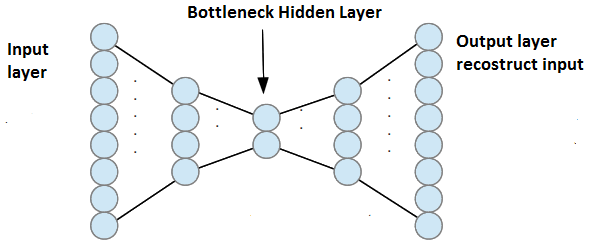
\psfig{file=autoencoders.png, width=0.6\textwidth}}
			\end{figure}
			\newpage
			
		\section{Work}
			The work done has the goal to verify whether the use of a Deep AE to accomplish the embedding(the n-dimensional node representation) lead to an improvement in performances, wrt. the embedding created by Word2Vec-algorithm.
			
			\begin{quote}
				\centering
				\textsc{finish}
			\end{quote}
			
			\subsection{Inspiration}
			\textit{Structural Deep Network Embedding} (SDNE) is a paper that covers the idea of reducing the data saved for each node in a network but maintaining good efficacy in reconstructing the network.\\
			The approach described in this paper it's related to completely known graphs, which isn't our case. In fact SDNE, as starting representation for each node utilizes its adjacency list in vector form:
			$$ S_{k} = [s_{1}, ... , s_{n}] $$
			$$ s_{i} > 0 \iff (v_{k},v_{i})\in E $$\\
			with $E$ being the set of edges of the graph, $S_{k}$ the representation relative to the node $v_{k}$ and $S$ the input for the NN. This representation is \textquotedblleft compressed" by the Deep AutoEncoder extracting a lighter dataset that can be very useful when dealing with huge graphs.\\
			Since the state of the graph is completely unknown to us, the idea is to replicate the same process utilising a slightly different way to identify nodes:
			\begin{equation}
			\begin{aligned}
			& S_{k} = [s_{1}, ... , s_{n}]\\
			& s_{i} = count(v_{k},v_{i})\\
			& count(u,v) =
			\begin{cases}
			c & \text{if the pair } (u,v) \text{  appears } c \text{ times in the cascades}\\
			0 & \text{if it never appears}\\
			\end{cases}\\
			\end{aligned}
			\end{equation}
			This list of values resembles a traditional adjacency list, but it's completely inferred by the cascades without any assurance on the truthfulness of the guesses.\\
			
			\subsection{Note on cascades and pairs of nodes}
			As previously said, short cascades gives us more information and more accuracy in prediction.\\
			Taking in example the case of the Twitter dataset, cascades are list of users that used a certain hashtag; in a small cascade we observe few people using the same hashtag, and so we can guess with fairly high confidence that they must follow each other because they saw the hashtag from each other. On the other hand the information is very local and doesn't cover the situation about the interconnection between communities and/or less evident grades of connection.\medskip\\
			The threshold $\lambda$ of the length of the cascades involved into the process of learning becomes an hyperparameter of the procedure. An expected phenomenon bound to the variation of $\lambda$ is that the lower it is, the more accurate will be the predictions, but the fewer arcs will be possible to infer. On the contrary, the exact opposite happens as $\lambda$ increases.
			
			\begin{algorithm}[H] % enter the algorithm environment
				\caption{Generate the pairs of nodes starting from a set of cascades} % give the algorithm a caption
				\label{alg1} % and a label for \ref{} commands later in the document
				\begin{algorithmic} % enter the algorithmic environment
					\REQUIRE $C$ the set of cascades, $\lambda$ the length threshold
					\ENSURE $CD$ the co-occurrence dictionary
					\STATE $C \gets$ sort\_by\_length(C)
					\STATE $CD \gets dict(\text{key:} (int,int), \text{value:} int)$
					\FORALL{$c \text{ in } C \text{ such as } c.length() \le \lambda$}
						\FOR{$i$ from  $1$ to $c.length()$}
							\FOR{$j$ from $i+1$ to $c.length()$}
								\STATE update\_occurrence($CD,pair(c[i],c[j])$)
							\ENDFOR
						\ENDFOR
					\ENDFOR
				\end{algorithmic}
			\end{algorithm}
			
			\begin{algorithm}[H] % enter the algorithm environment
				\caption{Given a key, increases the value by one of a Dictionary} % give the algorithm a caption
				\label{alg2} % and a label for \ref{} commands later in the document
				\begin{algorithmic} % enter the algorithmic environment
					\REQUIRE $D$ the dictionary, $k$ the searched key
					\ENSURE the increment of the counter(the value) related to $k$
					\IF{$D.$lookup($k$) $\neq$ NULL}
						\STATE $D[k] \gets D[k]+1$
					\ELSE
						\STATE $D[k] \gets 1$
					\ENDIF
				\end{algorithmic}
			\end{algorithm}
			
			\subsection{Deep Autoencoder Training}
			The autoencoder learns to reproduce its input-data batches effectively, throughout different epochs of training specializing in compressing reproductions of the fixed dataset. Once the training is completed, the middle-layer of the neural network gives us the representation for a given input; this can be used as a substitute of the Word2Vec encoding for the network-inference task. The inference and evaluation process is done the same way it was executed in the paper DeepInfer.
			
				\subsubsection{Motivation}
				The main reason why this attempt of improvement has been tried is because of the different architecture that offers the embedding.\\
				In \textit{Word2Vec}, the model tries to enforce similar representation for words in the same context-window trough a shallow Autoencoder trained with the goal of predicting couples of words.\\
				But as explained in SDNE, it's hard to capture highly non-linear structure (in this case the structure of the network) with a representation learnt using a shallow model (Word2Vec). Hence, the multiple levels of the autoencoder should learn the complexity of the structure of the network, and efficiently construct a good representation for each vertex.
				
				\subsubsection{Results}
				Three different datasets were used to validate this procedure. They all represent social graphs of different nature, but the procedure can be applied to every kind of graph that has some tangible and visible interaction that occurs between its nodes. The first two dataset are medium-small graphs, while twitter tends to be bigger. The nodes represent users/people and the arcs stand for, respectively, the interchange of emails in an european institute of research, friends on facebook and following on Twitter.
				\begin{center}
					\begin{tabular}{l | c | c}
						\textbf{Dataset} & \textbf{Nodes} & \textbf{Edges} \\
						email-Eu & 1005 & 25571 \\
						social circles: facebook & 4039 & 88234 \\
						twitter (original) & 595460 & 14273311\\
						twitter (subsampled) & 100000 & 1278006
					\end{tabular}	
				\end{center}
			
				\bigskip
				For the first two datasets the cascades (interactions between the nodes) were generated starting from the actual graph and taking random walks of variable length: the latter parameter was generated with an exponential distribution ($\lambda e^{-\lambda x}$ for $x\ge 0$) starting from each vertex of the graph multiple times. On the other hand, for Twitter I already had a set of actually observed cascades.\smallskip\\
				The shapes of the different autoencoders aimed to compress by orders of magnitude the inferred \textquotedblleft \textit{adjacency list}\textquotedblright in order to squeeze similar nodes close together. Here follows the shapes of the autoencoders:
				\begin{center}
					\begin{tabular}{l | c}
						\textbf{Dataset} & \textbf{Shape} \\
						email-Eu & [1005 $\rightarrow$ 250 $\rightarrow$ 10 $\rightarrow$ 250 $\rightarrow$ 1005] \\
						social circles: facebook & [4039 $\rightarrow$ 250 $\rightarrow$ 10 $\rightarrow$ 250 $\rightarrow$ 4039]  \\
						twitter (subsampled) & [500k $\rightarrow$ 10k $\rightarrow$ 128 $\rightarrow$ 10k $\rightarrow$ 500k]
					\end{tabular}	
				\end{center}
				The whole Twitter dataset had some troubles of treatability linked to the size of the set of nodes, that made impossible to fit in memory the data needed to train the Neural Network (that itself was too large). Hence the dataset has been sized down to about a sixth of the original nodes for manageability purposes.\\
				The results are shown in the table below.
				
				\begin{center}
					\begin{tabular}{l | c | c | c | c }
						\textbf{Dataset} & \textbf{True Positives} & \textbf{False Positives} & \textbf{False Negatives} & \textbf{True Negatives}  \\
						email-Eu &  8067 & 314711 & 16862 & 669380\\
						social circles: facebook & 74405 &	13720121 & 13829 & 2501127\\
						twitter (subsampled) & 1278006 & 4998671994 & 0 & 0
					\end{tabular}	
				\end{center}
				\hskip0.0cm
				\begin{tabular}{l | c | c}
					\textbf{Dataset} & \textbf{Precision} & \textbf{F1 score} \\
					email-Eu &  0.026 & 0.046\\
					social circles: facebook & 0.005 &	0.011\\
					twitter (subsampled) & 0.00025 & *
				\end{tabular}	
			
			
				\paragraph{Small Datasets:} small datasets performed badly; some hypothesis can be made about the lack of training data or the fact that being such small networks, they are influenced a lot by fluctuations due to the randomness of the source (humans).
				\paragraph{Twitter dataset:} to explain the very controversial results obtained by this dataset, is due a look on the embedding of the node. The representation of the vertexes of the net consist mostly of 0s and 1s, interlapped by rare floating point values between those two. This means that the autoencoder learnt a good way of reproducing the lists of 100k integers really well, basically mapping them on keys of dimension 128. This made completely fail the goal of the process, and created very similar representation for each node, but the network was still able to reconstruct accurately the inputs.\\
				Even the inputs were kind of particular: since they were constructed starting from the cooccurrence of pairs in the cascade, the nodes never found many matches to cover the majority of the nodes, leaving the most part of their so called \textquotedblleft adjacency-list\textquotedblright empty (0 values). \bigskip \\
				The method as it is isn't effective at all, and the accomplishment done by the Autoencoder has been merely to select relevant values acting as a compression algorithm, but failing at giving good embedding for the Network Inference Task. Furthermore, the trained NN had as objective to be able to reconstruct adjacency lists that weren't accounting the actual proximity between nodes in the new representation. If two different nodes had similar neighbours, they would have also similar representation but this doesn't imply that they are neighbours too. This assumption can be made on graphs with very densely connected communities and very few inter-community links.
				
				\newpage
			\subsection{Practical issues}
			- python problems (memory efficiency)\\
			- adaptments\\
			- c++ introduction\\
			- problems with c++\\
			
			Since the beginning of this thesis, the language that I've used is Python. Reproducing the results shown in DeepInfer wasn't a problem at all, due to the light-weight of the computations needed since the \textquotedblleft heavy\textquotedblright work consisted on generating the embedding with \textit{Word2Vec}. The process took some minutes but one of the pros of the previously cited method is the lightness, given that the NN is shallow.\\
			On the other hand, the Autoencoder carries some not irrelevant dimensions/memory issues; since the input and the output layers can be very large, adding fully-connected layers in this kind of NN pumps up the amount of resources needed to handle the whole network through the training sections.\\
			Moreover, Python has some serious issues regarding memory efficiency in their data structures causing the work on big datasets really hard, since the data that should be fed into the net takes up much more memory than it should, leaving less resources to handle the Neural Network. A small example of this kind of problem is shown in the table below:\bigskip \\
			\textit{Allocation of $10^{9}$ integers}\\
			\vspace{0.8cm}
			\begin{centering}
				\begin{tabular}{l | c}
					\textbf{Data Structure} & \textbf{Memory Occupancy}\\
					Python: standard list [] & ~7.48 GB \\
					Python: array.array & over 30 GB\\
					C++: vector$<$int$>$ & 3.78 GB
				\end{tabular}
			\end{centering}
			\newline
			The lower bound for storing that amount of integer values is accomplished by C++, that also provides very efficient and fast operations; Python requires a lot more resources in order to be time-efficient (array.array) and the simplest implementation of the list takes up almost the double of the memory needed.\\
			As to be expected, using dictionaries and more complex data structures, matters get even worse.\smallskip\\
			While utilising the Twitter dataset (about 600000 nodes initially), I had to subsample the set of nodes, since that just storing a Tensorflow Deep Autoencoder (fully connected layers with shape [500k $\rightarrow$ 10k $\rightarrow$ 128 $\rightarrow$ 10k $\rightarrow$ 500k]) couldn't be done on the machines that I had access to (100GB RAM). Hence, I took a subsample ok 100k nodes in order to be able to fit the Neural Network in memory.\\
			As mentioned before,
			\begin{quote}
				\centering
				\textsc{To be finished}\\
			\end{quote}
			
			
			\newpage
			
	\section{Bibliography}
	\begin{thebibliography}{10}	
		
		\bibitem{deepinfer}
		Zekarias T. Kefato and Nasrullah Sheikh and Alberto Montresor, 2017, \textit{\textsc{DeepInfer}: Diffusion Network Inference through Representation Learning}, KDD2017, Halifax, Nova Scotia, Canada
		
		\bibitem{deeplearningbook}
		Ian Goodfellow and Yoshua Bengio and Aaron Courville, 2016, \textit{Deep Learning}, MIT Press, http://www.deeplearningbook.org
		
		\bibitem{sdne}
		Daixin Wang, Peng Cui and Wenwu Zhu, 2016, \textit{Structural Deep Network Embedding}, KDD ’16, San Francisco (CA), USA
		
		\bibitem{twitterdata}
		\textbf{Twitter Dataset}: Lilian Weng, Filippo Menczer, and Yong-Yeol Ahn. \textit{Virality Prediction and Community Structure in Social Networks}. Nature Scientific Report. (3)2522, 2013.
		
		\bibitem{facebookdata}
		\textbf{Facebook Dataset}: J. McAuley and J. Leskovec. Learning to Discover Social Circles in Ego Networks. NIPS, 2012.
		
		\bibitem{emaildata}
		\textbf{Email Dataset}: Hao Yin, Austin R. Benson, Jure Leskovec, and David F. Gleich. "Local Higher-order Graph Clustering." In Proceedings of the 23rd ACM SIGKDD International Conference on Knowledge Discovery and Data Mining. 2017.
		
		
	\end{thebibliography}
			
\end{document}